
% !TEX root = main.tex
\section{Framework}
\label{sec:framework}

In this section, we present the problem and our solution to it.

\subsection{Problem Statement}

For a given pair of entity, we formalize the problem of explaining the relationship between them as finding the attribute with a probability ranking.
More formally, given an entity pair $ \langle e_1, e_2 \rangle $, we want to find
\begin{equation}
\argmax_a P(a|\langle e_1,e_2 \rangle)
\end{equation},
where $P(a| \langle e_1, e_2 \rangle )$ is the probability that attribute $a$ is an attribute between two entities.
For example, for entity \at{Bill Gates, Microsoft}, \at{founder, board} are among the most probable relations.
However relation like \at{key people} is not that typical. We give notations used in this paper in Table...

\subsection{Concept based Inference}
Thus our problem is reduced to the estimation of $P(a| \langle e_1, e_2 \rangle )$.
The direct estimation is difficult since no such samples are available.
We resort to the concepts of entities to bridge the inference from entity pair to their relationship.
The rationality comes from the observation that it is the concept determines the relationship between entities.
For example, \at{<Washington, USA>} can be best explained by \at{CapitalOf} attribute, which essentially is determined by the concept pair \at{<Capital City, Country>}.
In other words, a certain relationship can be considered as generated by a corresponding concept pairs.
The entities pairs that belongs to the same concepts pairs share the same relationship explanation.
Continue the previous example, \at{<Beijing, China>} is clearly another example of entity pairs belonging to \at{<Capital, Country>} that can be explained by the \at{CapitalOf} attribute.

Using concept pairs as intermediate random variables, inference from entity pair to attribute can be restated as the following equation:
\begin{equation}
\label{eq:target}
\argmax_a \sum_{c_i\in C_1 , c_j \in C_2 }P(a|\langle c_{i},c_{j}\rangle)\times P(\langle c_{i},c_{j}\rangle|\langle e_{1},e_{2}\rangle),
\end{equation}
where $P(a|\langle c_{1},c_{2}\rangle)$ is the probability that attribute $a$ is relationship between the concept pair
and $P(\langle c_{i},c_{j}\rangle |\langle e_{1},e_{2}\rangle)$ is the probability that $\langle c_1, c_2\rangle$ is the concept pair of $ \langle e_1, e_2 \rangle $.
$P(a| \langle c_{1},c_{2} \rangle )$ can also be regarded as the {\it typicality} of attribute $a$ given the concept pair.
For the same concept pairs, some attribute is more typical than another one.
For a pair \at{<artist, country>}, the attribute \ac{hometown} is more typical than \ac{education}
For a given entity pair, their exists a distribution of concept pairs and some concept pair is better to characterize the concept of the entity pair than others.
As example,  for \at{<apple, Steve Jobs>},  \at{<company, entrepreneur>} deserves a higher probability than \at{<food, name>}.
$P( \langle c_{i},c_{j} \rangle | \langle e_{1},e_{2} \rangle )$ can also be considered as the typicality of the concept pair for the given entity pair.


Another benefit of concept-level estimation is that it can reduce the computation cost.
In general, the number of concept pairs is significantly less than that of entity pairs.

\subsection{Target Expand}
Given, Eq~\ref{eq:target}, the estimation of $P(a| \langle e_1,e_2 \rangle )$ boils down to 2 parts:
\begin{enumerate}
\item $P(a| \langle c_{1},c_{2} \rangle )$: Calculating the typicality of an attribute for a concept pair.
\item $P( \langle c_{i},c_{j} \rangle | \langle e_{1},e_{2} \rangle )$: Calculating the typicality of the concept pair for an entity pair.
\end{enumerate}

Using Bayesian rules, $P(a| \langle c_{1},c_{2} \rangle )$ can be restated in Eq.\ref{eq:target_expand1}:
\begin{equation}
\label{eq:target_expand1}
\begin{split}
P(a|\langle c_{1},c_{2} \rangle) &= \frac{ P(\langle c_{1},c_{2}\rangle|a)\times P(a) }{ P(\langle c_{1},c_{2}\rangle) }
%&=\frac{ p((c_{1},c_{2})|a)\times P(a) }{ \sum{P( (c_{1},c_{2})|a^* )\times P(a^*)   } },
\end{split}
\end{equation},
where $P(a)$ is probability to observe an entity pair with attribute $a$.


\subsection{Estimation of $P(\langle c_1,c_2\rangle | \langle e_1,e_2\rangle)$ }
A straightforward estimation of $P( \langle c_{1},c_{2} \rangle | \langle e_{1},e_{2} \rangle )$ is as follows when we assume that the choice of concept for $e_1$ is independent of that for $e_2$:
\begin{equation}
\label{eq:target_expand2_naive}
\begin{split}
P(\langle c_{1},c_{2}\rangle |\langle e_{1},e_{2} \rangle) = P(c_1|e_1) \times P(c_2|e_2)
\end{split}
\end{equation} The rationality is that the typicality of a concept pair can be quantified as the product of their respective typicality of each concept given its corresponding entity.
However, the assumption does not always holds. For example, given an entity pair \at{<apple, steve jobs>}. The candidate concepts for \at{apple} are \at{\{fruit,company,...\}} and the candidate concepts for \at{steve jobs} are \at{\{entrepreneur, pc developer,...\}}. Obviously, the concept pair \at{<fruit, entrepreneur>} is meaningless in this case. Hence, we need to introduce a factor $\alpha(c_1,c_2)$ into Eq.~\ref{eq:target_expand2_jr} to quantify the tendency that the two concepts are the appropriate concepts of the attribute. Thus, we have the following improved estimation:
\begin{equation}
\label{eq:target_expand2_jr}
\begin{split}
P(\langle c_{1},c_{2}\rangle |\langle e_{1},e_{2} \rangle) = \alpha(c_1,c_2) \times P(c_1|e_1) \times P(c_2|e_2)
\end{split}
\end{equation}


One simple simple estimation of $\alpha(c_1,c_2)$ is using the prior probability of $\langle c_1, c_2\rangle$, i.e., $P(\langle c_1,c_2\rangle)$. This is reasonable since the true concept pair for an entity pair in general has a larger probability than 
a false concept pair. 
Thus the objective function is reduced to Eq.~\ref{eq:simple_obj} when Eq.~\ref{eq:rel_jdp} holds


%the version of the  where we
%A simple estimation of $\alpha(c_1,c_2)$ is using the prior probability of $\langle c_1, c_2\rangle$.
\nop{
This section is devoted to calculating $s(c_1,c_2)$ of $P( \langle c_{1},c_{2} \rangle | \langle e_{1},e_{2} \rangle )$ in Eq.~\ref{eq:target_expand2_jr} and $P( \langle c_{1},c_{2} \rangle |a)$ of $P(a| \langle c_{1},c_{2} \rangle )$ in Eq.~\ref{eq:target_expand1}.

According to $P( \langle c_1,c_2 \rangle | \langle e_1,e_2 \rangle )$, we can only at concept level indicate the implicit relationship.
$P(a| \langle c_{1},c_{2} \rangle )$ retrieves the most probable alias of relation given the concept pair.
Thus our objective function solve 2 problems,
1) give out the most probable relation alias for a concept pair.
2) when multiple relations exist in one concept pair, decide which one is most typical.
}

\begin{equation}
\label{eq:simple_obj}
 \argmax_a \sum_{c_i\in C_1, c_j\in C_2} P(\langle c_{i},c_{j}\rangle |a)\times P(a)\times P(c_i|e_1)\times P(c_j|e_2)
\end{equation}

\begin{equation}\label{eq:rel_jdp}
  \alpha(c_1,c_2) = P(\langle c_1, c_2\rangle)
\end{equation}


%\xch{(c1,c2) is only one aspect, any other factor can affect the relation?}
%\xch{ in s(c1,c2), we only considered the attribute part, other signals such as entity co-occurrence of <e1,e2> can be considered }

\nop{
Eq.~\ref{eq:simple_obj} means finding the most probable attribute of $(e_1,e_2)$ by looking at their best concept pair, and find the most probable attribute given the concept pair.




Combining all these together, the ultimate optimization objective is described in Eq.~\ref{eq:target_expand_all}

\begin{equation}
\label{eq:target_expand_all}
\begin{split}
 \argmax_a \sum_{c_i\in C_1, c_j\in C_2}\frac{ p((c_{i},c_{j})|a) P(a)\alpha(c_i,c_j) P(c_i|e_1) P(c_j|e_2) }{ \sum_{a_k}{P( (c_{i},c_{j})|a_k) P(a_k)   } }
\end{split}
\end{equation}
}



\subsection{Solution Framework}
The main framework is illustrated in Figure~\ref{fig:framework}, which consists of two major components: the online computation and offline training. We refer to our system as \ac{Entity Relation Finder(ERF)}.
ERF takes an entity pair as input and find its most plausible relation as the result.
As a preprocessing step, we first directly lookup the attribute for the query entity pair from DBpedia.
If DBpedia has SPO triples connecting the entity pair, we direct return the predicate as the answer.
Otherwise, the procedure goes into the online computation component.
The online component calculates $ P(a|  \langle e_1,e_2 \rangle  )$ for each candidate attribute in $A$ by Eq.~\ref{eq:simple_obj} and return the maximal one as the answer attribute. To compute Eq.~\ref{eq:simple_obj}, we need to compute $P(c_1,c_2|a)$, $P(a)$, $P(c_1|e_1)$ and $P(c_2|e_2)$. We compute $P(c_1|e_1)$ and $P(c_2|e_2)$ on demand, that is, in the online component. We will explain it later in Section~\ref{sec:conceptualization}.. 
In the offline part, we compute $P(c_1,c_2|a)$ and $P(a)$ by leverage the SPO triples in DBpedia and isA relationships in Probase.
We elaborate their computation detail in Section ..

\begin{figure}[!ht]
\centering
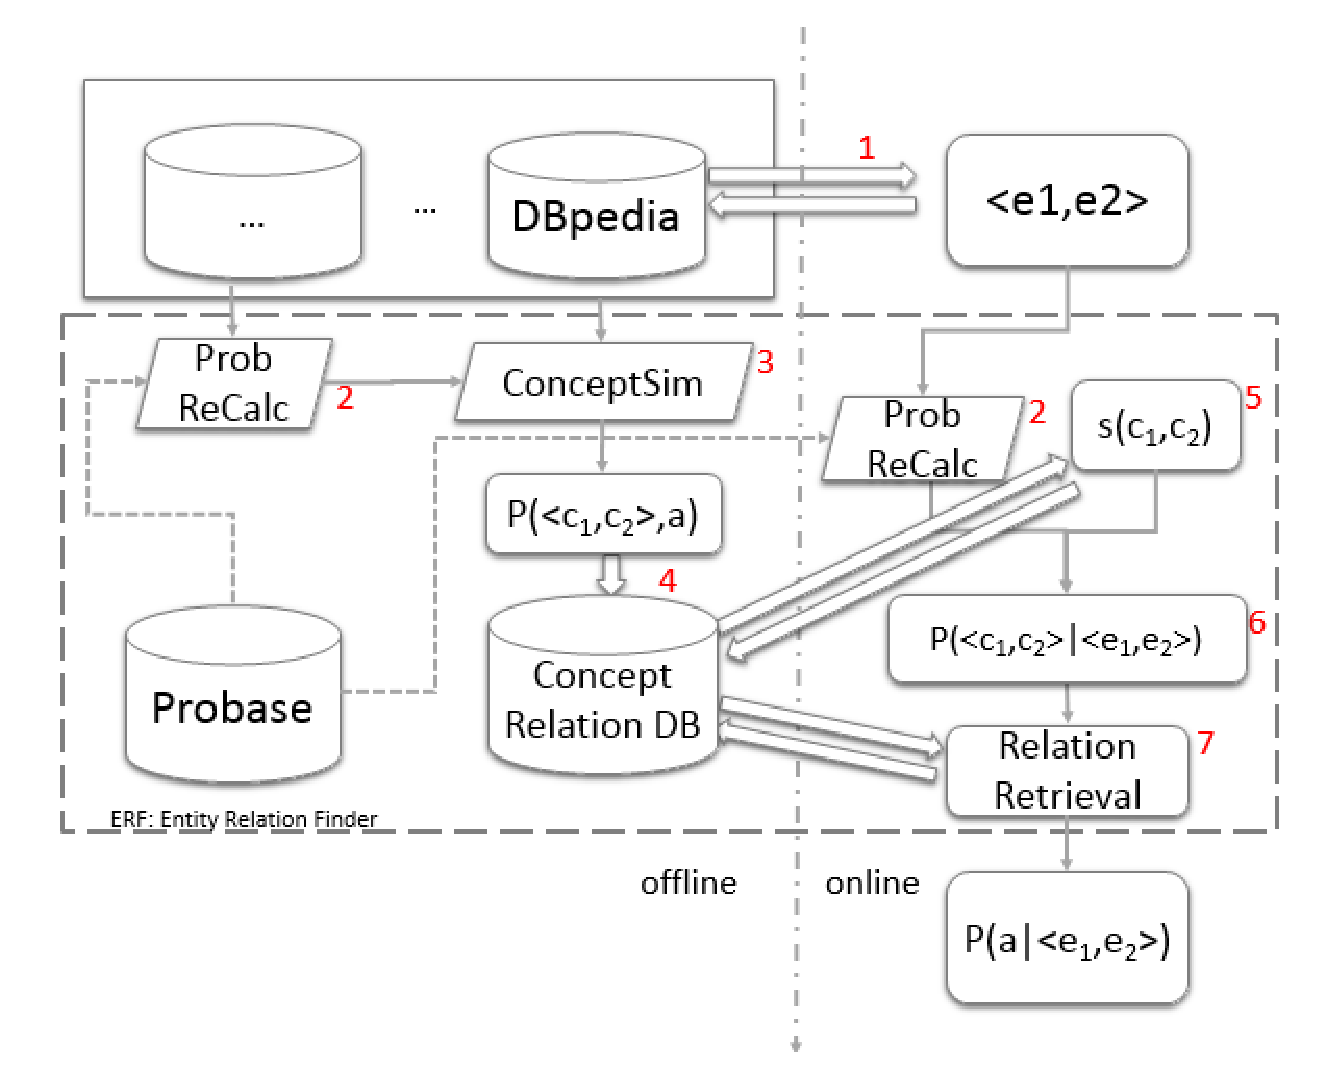
\epsfig{file=resources/framework.eps,width=\columnwidth}
\caption{System Framework of ERF}
\label{fig:framework}
\end{figure}


\nop{
In the online part, we first directly lookup the attribute for the query entity pair from DBpedia.
If DBpedia has no the exact the SPO triples connecting the entity pair, we In $step 2$, the concepts of the entities in knowledge bases are calculated(i.e. $P(c_i|e_i)$ in Eq.~\ref{eq:target_expand2_jr}).
The detailed process in in
$Step 3$ is the training process, $P( \langle c1,c2 \rangle ,a)$ is calculated for every attribute $a$ in Eq.~\ref{eq:pccga}.
The result is then stored in Concept Relation DB in $step 4$.

In  $step 1$, when a query entity pair comes, knowledge bases such as DBpedia are looked up and the exact relationship, if exists, is answered in the first place.
If nothing is found in $step 1$, the process will go into the ERF solution.

We first conceptualize the 2 entities in $step 2$.
The concept similarity score in Eq.~\ref{eq:target_expand2_jr}) is retrieved from the Concept Relation DB in $4$.
%\ref{eq:pcca}
So far we get everything for calculating Eq.~\ref{eq:target_expand2_jr}).
Then in $step 7$ we query the concept relation database and get the relation between concept pairs, specifically, $P(a| \langle c_1,c_2 \rangle )$ in Eq.~\ref{eq:target_expand1}.
Finally, we achieve the final object by combining all these together to infer $\argmax P(a| \langle e_1,e_2 \rangle )$ from Eq.~\ref{eq:target_expand_all}.
We return the the attribute owning the maximal score as the explanation for the relationship between the entity pair.

When no direct edges are found, we use the shortest path on the concept attribute graph to find the middle concepts, then the problem automatically reduced to relation explanation of several pairs of entities, discussing which is beyond the coverage of this paper.
}


%\paragraph{Paper Orgnization}
%The rest of the paper is organized as follows, Section~\ref{sec:conceptualization} describe how to derive $P(c|e)$ leveraging the \xch{basicness} of concept, Section~\ref{sec:fafa} is devoted to the offline calculation of $JD(c_1,c_2)$ and $P((c_{1},c_{2})|a)$.


\begin{table}[htbp]
  \centering
  \caption{Notation Table}
    \begin{tabular}{rr}
    \toprule
    notation & meaning \\
    \midrule
    $a$     & attribute \\
    $e_i$  & entity \\
    $c_i$  & concept \\
    $n(\cdot)$  & CountOf \\
    $h(\cdot)$ & HeadOf \\
    $c_h$  & head concept \\
    $\bar{C}$ &  head concept set\\
    $c_l$  & long concept \\
    $\langle e_1,e_2 \rangle$ & entity pair\\
    $\langle c_1,c_2 \rangle$ & concept pair\\
    $\alpha(\cdot,\cdot)$ & joint factor\\
    $T_k$ & E$A$E tuple with $a_k$ as $A$\\
    \bottomrule
    \end{tabular}%
  \label{tab:notation}%
\end{table}%


%First,we do conceptualization.
%
%Next,Judge whether the 2 entities are conceptually same
%
%Then, there are 2 cases of the CanBeExplained function:
%
%\begin{itemize}
%\item Explain 2 conceptually similar entity
%
%\begin{table}[htbp]
%  \centering
%  \caption{conceptually similar entity}
%    \begin{tabular}{rr}
%    \toprule
%    entity & concept \\
%    \midrule
%    Steve jobs & Person \\
%    Bill Gates & Person \\
%    \bottomrule
%    \end{tabular}%
%  \label{tab:addlabel}%
%\end{table}%
%
%
%\item Explain 2 conceptually different entity
%% Table generated by Excel2LaTeX from sheet 'Sheet1'
%\begin{table}[htbp]
%  \centering
%  \caption{Add caption}
%    \begin{tabular}{rr}
%    \toprule
%    entity & concept \\
%    \midrule
%    Mona Lisa & Painting \\
%    Renaissance & Period \\
%    \bottomrule
%    \end{tabular}%
%  \label{tab:addlabel}%
%\end{table}%
%
%Note that the concept here are not unique.
%
%\end{itemize}
%
%
%Last, We rank all the explanations in each step.
%
%
%

\section{Offline Learning}
In this section, we elaborate how we estimate $P(a)$ and $P( \langle c_{1},c_{2} \rangle |a)$ from knowledge bases DBpedia and Probase.

\subsection{Computation of $P(a)$}
All the probabilities can be estimated from the SPO(\at{<subject, predicate, object>} ) triples such as \at{<Bill Gates, board, Microsoft>}  in DBPedia.
Let $ \langle e_i, a_k, e_j \rangle $ be an SPO triple in DBPedia.
The triple means that entity $e_i$ has a attribute $a_k$ with value or object as $e_j$.
We only consider the SPO triples with O as entity, this attributes such as \at{height,year} are removed in the first place.
Let $E$ be the set of all entities and $A$ be the set of all attributes.
Let $T=\{ \langle e_i, a_k, e_j \rangle  | e_i,e_j\in E, a_k\in A\}$ be all triples in DBpedia.
For a given attribute $a$, $P(a)$ can be computed by
\begin{equation}
\label{eq:pa}
P(a)=\frac{n(a)}{\sum_{a_k\in A}{n(a_k)}},
\end{equation}
where $n(a)$ is the count of triples in $T$ with attribute $a$.


\subsection{Calculating $P( \langle c_{1},c_{2} \rangle |a)$ }

Our basic idea is use collective inference to disambiguate concepts pairs.
Next, we show how to learn $\alpha(c_1,c_2)$ from training data.
The purpose of $\alpha$ is to prune false concept pairs. Hence, we need to 
assign a value close to zero for these false concept pairs. 
The baic principle is that 
(1)A false concept pairs only exits for a small part of
entity pairs that has the attribute.
(2) A true concept pairs exits for most entity pairs of the attribute.
These principles imply that the aggregation over all entities pairs can remove the false concept pairs.
This step, as mentioned before, is mainly for concept level disambiguation purpose.

For a certain attribute $a_k$, there are many entity pairs connected by the attribute in the knowledge base.
We use these entity-attribute-entity instance to estimate the conditional probability of a concept pair given an attribute.
More formally, let $T_k=\{\langle e_i, a_k, e_j \rangle\}$ be all the triples in the knowledge base with attribute as $a_k$.
$P( \langle c_1, c_2 \rangle |a_k)$ is estimated as follows:
\begin{equation}
P(\langle c_1, c_2\rangle|a_k)= \frac{1}{|T_k|}\sum_{  (e_{i},a_k,e_{j})\in T_k } P(c_1|e_{i})P(c_2|e_{j})
\label{eq:pccga}
\end{equation}
It is not difficult to prove that $0\leq P( \langle c_1, c_2 \rangle |a_k)\leq 1$ and their sum over all concept pairs equals to 1.
Hence $P( \langle c_1, c_2 \rangle |a_k)$ is a probability estimation.

\begin{example}[Calculating $P( \langle {c_h}_{1},{c_h}_{2} \rangle  |a)$]
\label{exa:pggga}
As illustrated in Figure~\ref{fig:bipartite}, the process of calculating $P(({c_h}_{1},{c_h}_{2}) |a)$ is as follows.
Given \term{company} and \term{entrepreneur}, we sum up all $P(c_1|e_1)\times P(c_2|e_2) $ such as $P(Company|Microsoft) \times P(Entrepreneur|Bill Gates)$,
\end{example}


\begin{figure}[!htb]
\centering 
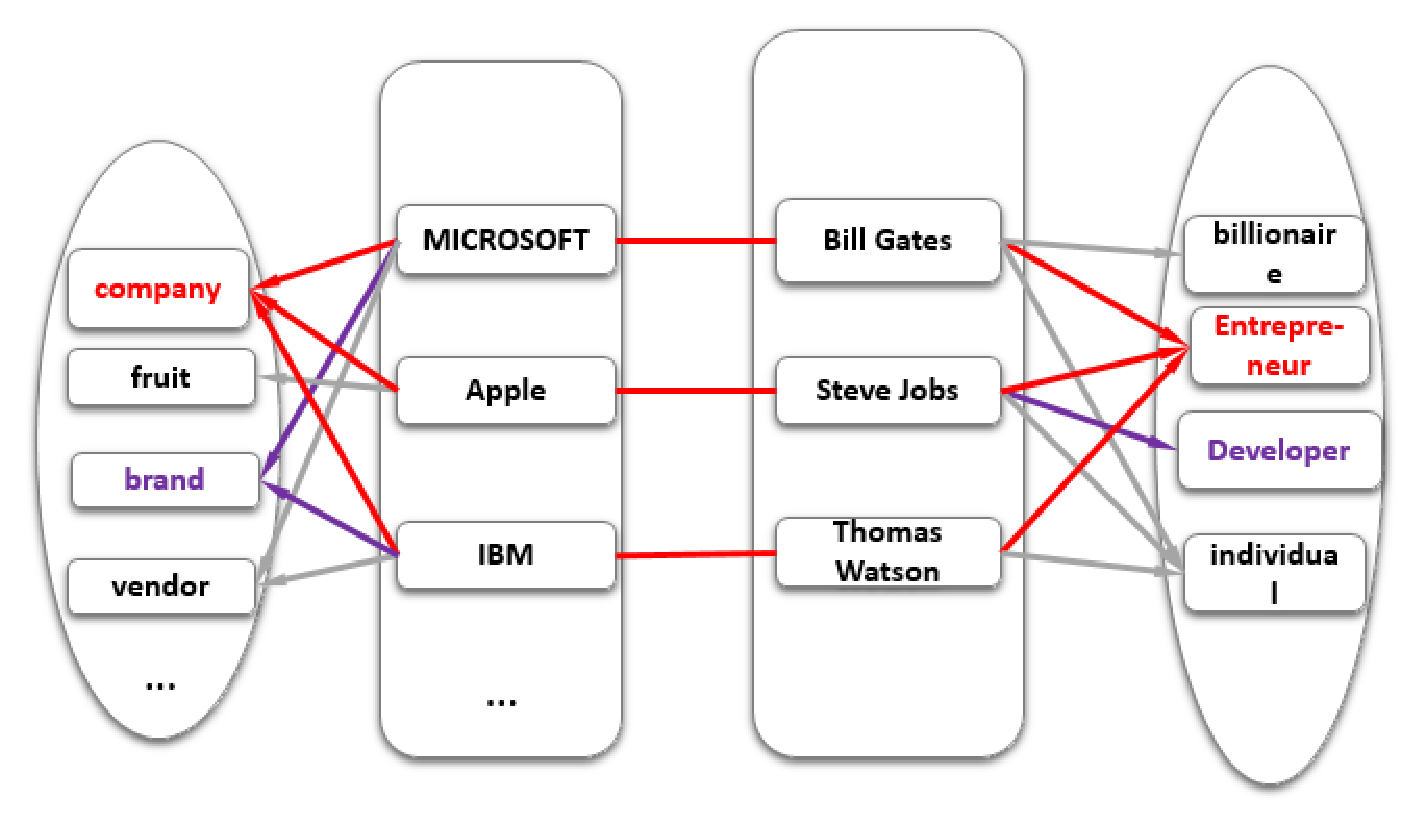
\epsfig{file=resources/ceaec.eps,width=\columnwidth}
\caption{Calculating $P(  \langle {c}_{1},{c}_{2} \rangle  | \term{FoundedBy} )$ } 
\label{fig:bipartite}
\end{figure}

\paragraph{Complexity analysis}

We first analysis the complexity of calculating $P(\langle c_i, c_j \rangle|a_k)$, manifest in Table.~\ref{tab:complexity}. The original one need to calculate $P(\langle c_i, c_j \rangle|a_k)$ for all $c \in C_1,C_2 $,while most of the concepts are, according to the power law, close to zero, which indicates the rationality of pruning.


\begin{table}[htbp]
  \centering
  \caption{Complexity Analysis}
    \begin{tabular}{rr}
    \toprule
    method & complexity \\
    \midrule
    original &  $O(|T_n||C_1||C_2|)$ \\
    topKpruned & $O(|T_n|K^2)$ \\
    \bottomrule
    \end{tabular}%
  \label{tab:complexity}%
\end{table}%


%%% Local Variables: 
%%% mode: latex
%%% TeX-master: "main.tex"
%%% End: 